\documentclass[tikz]{standalone}
\usepackage{tikz}
\usetikzlibrary{plotmarks}
\usetikzlibrary{math}

\usepackage{pgfplots}
\pgfplotsset{compat=newest}

\begin{document}
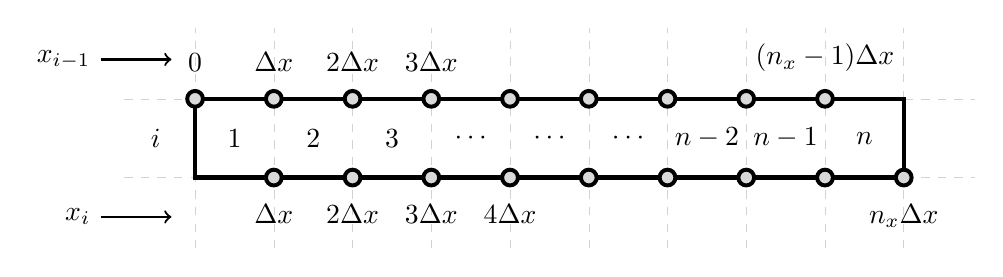
\begin{tikzpicture}
    % grid lines
    \draw[help lines, color=gray!35, dashed, step=1] (-0.9,-0.9) grid (9.9,1.9);
    \draw[ultra thick] (0,0) rectangle ++(9,1);
    % points above
    \draw[fill=gray!30, line width=0.5mm] (0,1) circle[radius=1mm] node[above=2mm, black] {$0$};
    \draw[fill=gray!30, line width=0.5mm] (1,1) circle[radius=1mm] node[above=2mm, black] {$\Delta x$};
    \draw[fill=gray!30, line width=0.5mm] (2,1) circle[radius=1mm] node[above=2mm, black] {$2 \Delta x$};
    \draw[fill=gray!30, line width=0.5mm] (3,1) circle[radius=1mm] node[above=2mm, black] {$3 \Delta x$};
    \draw[fill=gray!30, line width=0.5mm] (4,1) circle[radius=1mm];
    \draw[fill=gray!30, line width=0.5mm] (5,1) circle[radius=1mm];
    \draw[fill=gray!30, line width=0.5mm] (6,1) circle[radius=1mm];
    \draw[fill=gray!30, line width=0.5mm] (7,1) circle[radius=1mm];
    \draw[fill=gray!30, line width=0.5mm] (8,1) circle[radius=1mm] node[above=2mm, black] {$(n_x - 1) \Delta x$};
    % points below
    \draw[fill=gray!30, line width=0.5mm] (0+1,0) circle[radius=1mm] node[below=2mm, black] {$\Delta x$};
    \draw[fill=gray!30, line width=0.5mm] (1+1,0) circle[radius=1mm] node[below=2mm, black] {$2\Delta x$};
    \draw[fill=gray!30, line width=0.5mm] (2+1,0) circle[radius=1mm] node[below=2mm, black] {$3\Delta x$};
    \draw[fill=gray!30, line width=0.5mm] (3+1,0) circle[radius=1mm] node[below=2mm, black] {$4\Delta x$};
    \draw[fill=gray!30, line width=0.5mm] (4+1,0) circle[radius=1mm];
    \draw[fill=gray!30, line width=0.5mm] (5+1,0) circle[radius=1mm];
    \draw[fill=gray!30, line width=0.5mm] (6+1,0) circle[radius=1mm];
    \draw[fill=gray!30, line width=0.5mm] (7+1,0) circle[radius=1mm];
    \draw[fill=gray!30, line width=0.5mm] (8+1,0) circle[radius=1mm] node[below=2mm, black] {$n_x \Delta x$};
    % node identifiers
    \node at (-0.5,0.5) {$i$};
    \node at (-0.5+1,0.5) {$1$};
    \node at (-0.5+2,0.5) {$2$};
    \node at (-0.5+3,0.5) {$3$};
    \node at (-0.5+4,0.5) {$\cdots$};
    \node at (-0.5+5,0.5) {$\cdots$};
    \node at (-0.5+6,0.5) {$\cdots$};
    \node at (-0.5+7,0.5) {$n-2$};
    \node at (-0.5+8,0.5) {$n-1$};
    \node at (-0.5+9,0.5) {$n$};
    % series identifiers
    \draw[->, thick] (-1.2,1.5) node[left] {$x_{i-1}$} -- (-0.3,1.5);
    \draw[->, thick] (-1.2,-0.5) node[left] {$x_{i}$} -- (-0.3,-0.5);
\end{tikzpicture}
\end{document}
